\documentclass[12pt]{article}
\setlength{\textwidth}{17cm}
\setlength{\textheight}{24cm}
\setlength{\topmargin}{-2cm}
\setlength{\footskip}{1cm}
\setlength{\evensidemargin}{0cm}
\setlength{\oddsidemargin}{0cm}

\usepackage{allrunes}
\usepackage{amsmath}
\usepackage[magyar]{babel}
\usepackage[T1]{fontenc}
\usepackage[utf8]{inputenc}
\usepackage{fixltx2e}
\usepackage{multirow}
\usepackage{hyperref}
\usepackage{amsfonts}
\usepackage{amsthm}
\usepackage{amssymb}
\usepackage{indentfirst}

\usepackage[a4paper, bindingoffset=0.2in, left=1.2in,right=1.2in, footskip=.25in]{geometry}

\theoremstyle{plain}
\usepackage{graphicx}

%\usepackage{gensymb}
\usepackage{float}

%linkek 
\newcommand{\ndurl}[2]{\textit{\href{#1}{\underline{#2}}}}

%% New commands
\newcommand{\ket}[1]{\left| #1 \right >}
\newcommand{\bra}[1]{\left < #1 \right |}
\newcommand{\braket}[2]{\left < #1 \middle | #2 \right>}
\newcommand{\ketbra}[2]{\left | #1 \right> \left< #2 \right |}
\newcommand{\norm}[1]{\left{||} #1 \right{||}}
\newcommand{\commut}[2]{\left [ #1 , #2 \right]}

\newcommand{\dd}{\textrm{d}}

\newcommand{\mev}{~\textrm{MeV}}
\newcommand{\fm}{~\textrm{fm}}

%% Pauli matrices
\newcommand{\sigx}{\sigma_x}
\newcommand{\sigy}{\sigma_y}
\newcommand{\sigz}{\sigma_z}

\newcommand{\paulix}{
    \left( \begin{array}{cc}
        0 & 1 \\
        1 & 0
    \end{array}
    \right)
}
\newcommand{\pauliy}{
    \left( \begin{array}{cc}
        0 & -i \\
        i & 0
    \end{array}
    \right)
}
\newcommand{\pauliz}{
    \left( \begin{array}{cc}
        1 & 0 \\
        0 & -1
    \end{array}
    \right)
}

\renewcommand\thesection{\Roman{section}}

\begin{document}
\title{Optikai pumpálás}
\author{Olar Alex}
\date{}

\maketitle
\vfill
\begin{figure}[h!]
    \begin{center}
    
\includegraphics[width=0.7\textwidth]{./images/elte.eps}
    \end{center}
\end{figure}

\newpage

\tableofcontents

\newpage

\section{Mérés leírás}
\par A mérés során az optikai pumpálás jelenségét vizsgáltuk Rb atomokon, mely során meghatároztuk a folyamatra jellemző időállandókat és a Zeeman-effektus során a giromágneses faktort.

\vspace{.5cm}

\par A labor során Rb és Kr gázt tartalmazó kisülési csövet használtunk, az ebből kijövő elektromágneses hullámokat lineárisan polarizáltuk és $\lambda/4$-es lemezzel cirkulárisan polarizáltuk.

\vspace{.5cm}

\par A fényelnyelést fotodiódával detektáljuk, az adatokat Pythonban értékeltük ki.

\section{Elméleti háttér}

\par Egyensúlyban az egyes energiaszintek betöltöttségét a Boltzmann-eloszlás írja le.

\begin{equation}
\label{eq:1}
\frac{N_B}{N_A}= e^{-\frac{E_B-E_A}{kT}}
\end{equation}

\vspace{.3cm}

\par Három energiaszinttel elérhető populáció inverzió, mely során az A szintről a B szintre pumpáljuk, melyből a C szintre esnek le a gerjesztett elektronok. A szintekre jellemző, hogy $E_{B} > E_{C} > E_{A}$. Így közvetve elérhető a pumpálás egy harmadik szint beiktatásával.

\vspace{.5cm}

\par A mostani mérés során 4 energiaszintünk van, mágneses térben a Rb atom $3^2S_{1/2}$ és $3^2P_{1/2}$ nívója Zeeman-effektus szerint felhasad az elektron spinje szerint. A legalsó A energiaszintről a legfelsőbe (D) kerül a rendszer a gerjesztés hatására, majd alapállapotba, vagy egy felsőbb szintre (B) kerül. Így a betöltöttség A-n csökken és létrejött a pumpálás.

\vspace{.5cm}

\par A felírt folyamatok sebességét időállandókkal jellemezhetjük. $T_1$ jellemzi a pumpálás kikapcsolása esetén a B $\rightarrow$ A átmenetet, $T_p$ az A $\rightarrow$ D átmenetet, $\tau = (T_1^{-1}+T_p^{-1})^{-1} < T_1, T_p$ pedig a pumpálásra jellemző effektív karakterisztikus idő. Ezen kívül bevezethető még egy időállandó ($T_2$) amely a Zeeman-felhasadás megszűnésekor mérhető relaxációs idő.

\vspace{.5cm}

\par Először a $T_2$ és $\tau$ időállandókat határoztuk meg, amelyekhez figyelembe kell venni a Föld mágneses terét is. Ezután A és B közti energiakülönbségnek megfelelő energiájú (radiofrekvenciás) gerjesztéssel rezonanciát érünk el. Folyamatos pumpálással populáció-inverziót érünk el A és B közt, és amennyiben a radiofrekvenciás foton energiája pont a Zeeman-felhasadás energiakülönbségének felel meg, indukált emisszió hatására relaxál a rendszer, amely az elnyelt fényintenzitás növekvésében mutatkozik meg. Ezt a fotodióda által észlelt intenzitás csökkenésében jelenik meg. A Zeeman-felhasadás energiaszintjét \aref{eq:2}. egyenlet írja le.

\vspace{.5cm}

\begin{equation}
\label{eq:2}
\Delta E = \mu_Bg_FB \overset{!}{=}h\nu
\end{equation}

\vspace{.3cm}

\par A mágneses teret $B=B_0+b\sin(\omega t)$ alakban változtatjuk, ahol $b < B_0$. A szinuszos modulációnak köszönhetően periodusonként 0,1 vagy 2-szer történik rezonancia-átmenet. Leolvasási pontnak azt választjuk, amikor $\sin(\omega t)$ 0 értékénél, azaz periodusonként kétszer jelenik meg rezonancia, azonos időkülönbséggel. A mérést mindkét irányban elvégezzük, ezáltal a kettő átlagával a Föld mágneses terét ki tudjuk kompenzálni. A mérést 4 frekvencián végezzük, azokat egy külön antennával mérjük. A fenti képlet alapján így meghatározható $g_F$, külön-külön mindkét Rb izotópra.


\section{$\tau$ időállandó meghatározása}

\par A fotodiódán keletkező feszültséget oszcilloszkóppal mértük, a periodikus jelből kiválasztottam 6 olyan szakaszt,
ahol exponenciális görbe figyelhető meg (\ref{fig:1}. ábra). Ezekre az elmélet szerint számolt $n=n_0(1-\exp(-t/\tau))$-tól eltérően, (a szingularitást
elkerülendő) $f(x)=n_1 + n_2\exp(-t/\tau)$ görbét illesztettem, amelyből a $\tau$ összevont időállandó meghatározható.

%Abra
\begin{figure}[H]
\centering
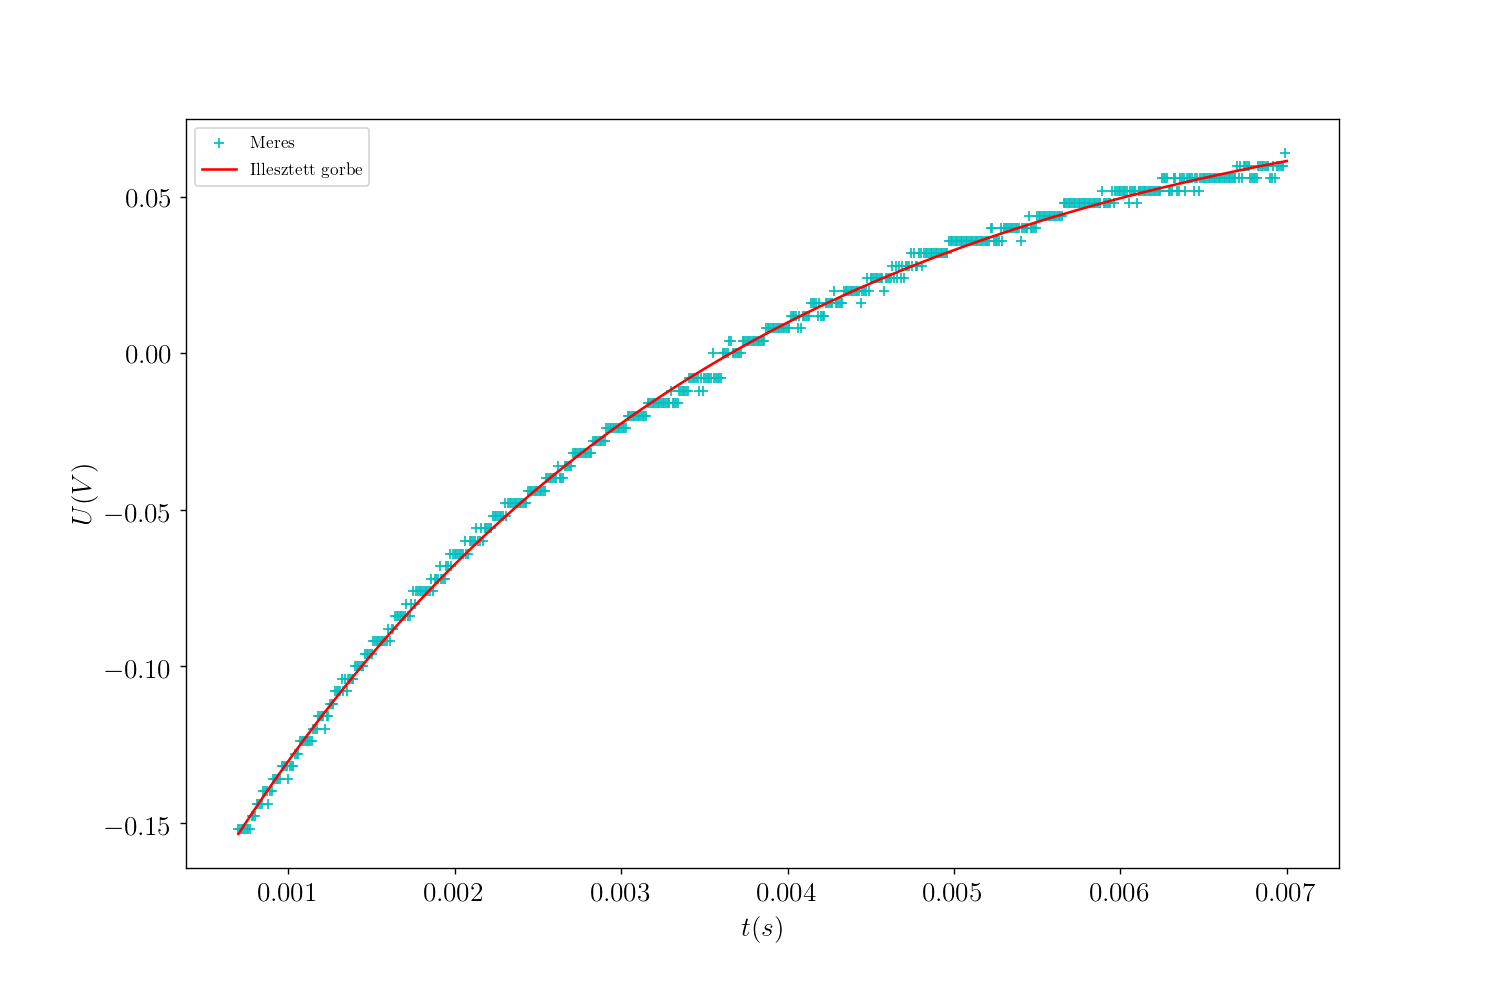
\includegraphics[width=0.99\textwidth]{j/tau22.png}
\caption{Helyes feszültség - idő görbe}
  \label{fig:1}
\end{figure}


\begin{table}[H]
\begin{tabular}{|c|c|c|c|c|c|c|c|}
 \hline
 $\tau_1$ & $\tau_2$ & $\tau_3$ & $\tau_4$ & $\tau_5$ & $\tau_6$ & $\overline{\tau}$ & $\sigma_{\tau}$ \\ \hline
 $0.00335$ & $0.0023$ & $0.00259$ & $0.00297$ & $0.00283$ & $0.00266$ & $0.00279$ & $0.00033$ \\ \hline
\end{tabular}
\caption{$\tau$ - átlag és szórás $n=6$ görbe alapján}
\label{tab:1}
\end{table}

\section{$T_2$ időállandó meghatározása}

\par Ezután megmértük a Zeeman felhasadás megszűnésekor bekövetkező relaxációs folyamat $T_2$ időállandóját.
\par Ehhez úgy állítottuk be a Helmholz-tekercsekre kapcsolt periodikus jel amplitúdóját, hogy keletkező
mágneses tér egyik félperiódusban pont kioltsa a Föld mágneses terét. Ebben a félperiódusban relaxáció
történik, ami a fotodiódán mérhtő intenzitáscsökkenésben mutatkozik meg (\ref{fig:2}. ábra). Erre exponenciális függvényt illesztve
megkaphatjuk a $T_2$ időállandót.

%Abra
\begin{figure}[H]
\centering
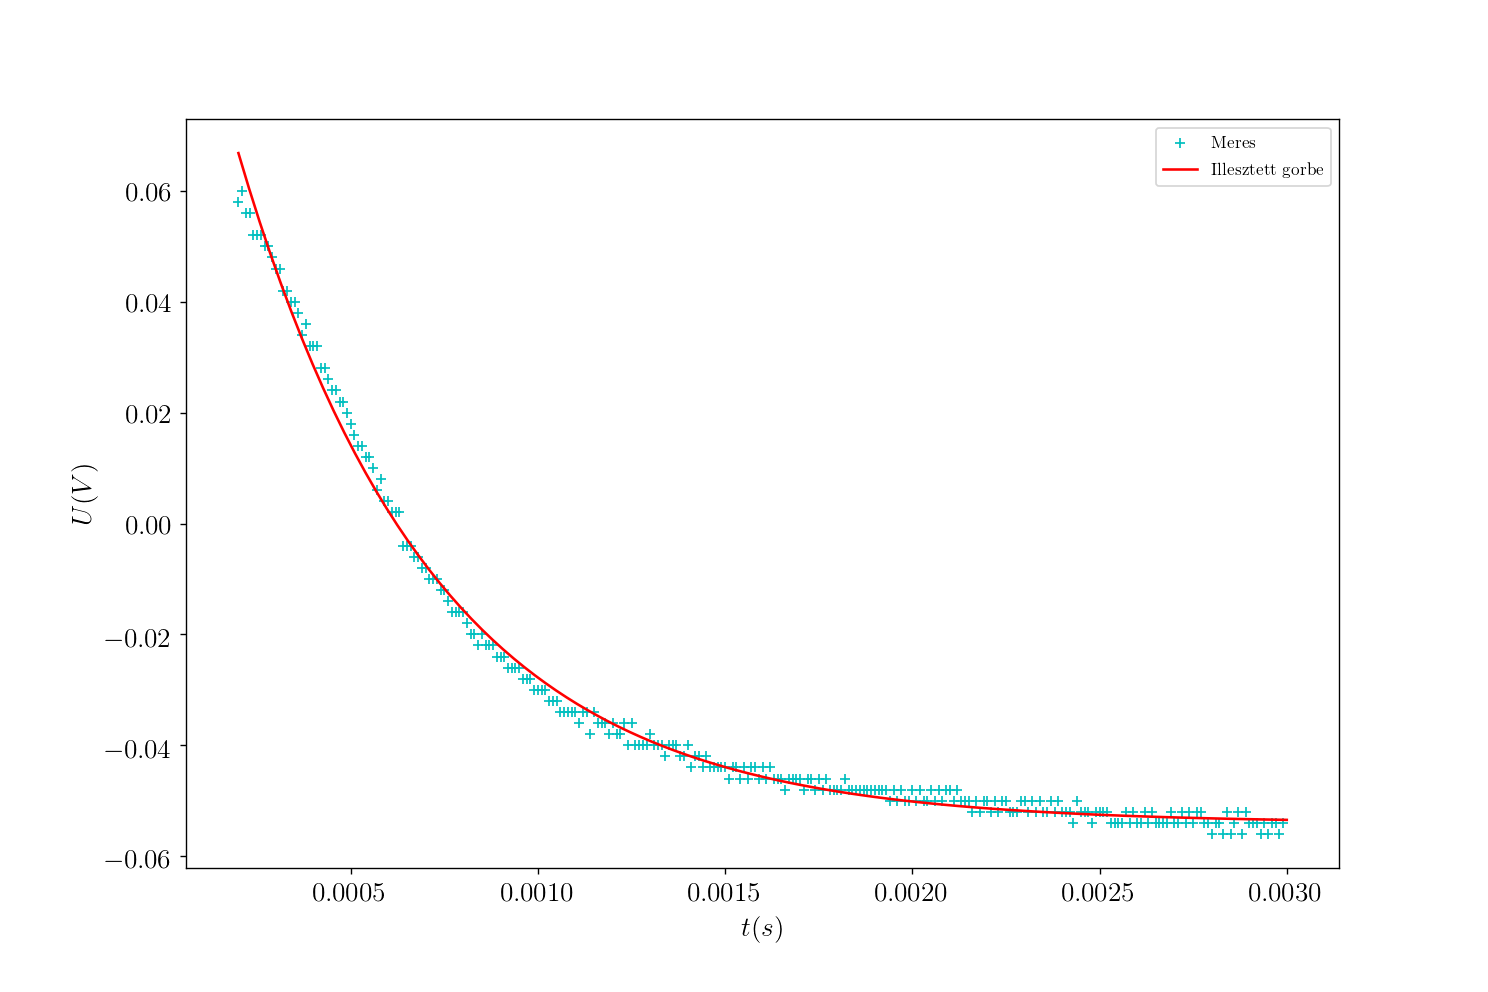
\includegraphics[width=0.99\textwidth]{j/t22.png}
\caption{Feszültség - idő}
\label{fig:2}
\end{figure}

\begin{table}[H]
\begin{tabular}{|c|c|c|c|c|c|c|c|}
 \hline
 $T_{21}$ & $T_{22}$ & $T_{23}$ & $T_{24}$ & $T_{25}$ & $T_{26}$ & $\overline{T_{2}}$ & $\sigma_{T_2}$ \\ \hline
 $0.000708$ & $0.000671$ & $0.000685$ & $0.000535$ & $0.000721$ & $0.000839$ & $0.000693$ & $0.000089$ \\ \hline
\end{tabular}
\caption{$T_2$ átlaga és szórása $n=6$ görbe alapján}
\label{tab:2}
\end{table}

%\input{intro-mod.tex}
\section{Rezonancia-átmenet vizsgálata \newline és giromágneses faktor meghatározása}
A rendszert négy frekvencián gerjesztettük radiofrekvenciás jellel. A mágneses indukcióvektor nagyságának meghatározásához felhasználtuk a Helmholtz-tekercsek paramétereit ($R = 19.3 cm, n = 80$), illetve a \ref{eq:3}-as egyenletet.

\begin{equation}
\label{eq:3}
B = \left(\frac{4}{5}\right)^{3/2} \frac{\mu_0nI}{R}
\end{equation}
A mért adatokat \aref{tab:3}. és  \aref{tab:4}. táblázat tartalmazza. A gerjesztési radiofrekvenciás jel frekvenciáját egy antenna segítségével oszcilloszkópon mértük, leszámolva adott idő alatt megjelenő periódusokat. A giromágneses faktor ($g_F$) éppen az $E(B\mu_B)$ egyenes meredeksége (\ref{fig:3}. ábra). A kapott giromágneses faktorok a két izotópra: $g_{F,1} = 0.5154 \pm 0.0012$ és $g_{F,2} = 0.3414 \pm 0.0004$.
A mérésből meghatározható a Föld mágneses terének az indukált B irányú vetülete (a két irányban mért B különbségének a fele), amely $B_{F} = (14.0\pm 0.8 )\mu T $-nak adódott.
\\ A kapott giromágneses faktorok jól közelítik az elméleti értéket. A vizsgált rendszerben $S = 1/2, J = 1/2, I_1 = 3/2, I_2 = 5/2$. Ekkor $g_J = 2$ adódik, ebből pedig $J=1/2$ esetén $g_F = \frac{g_J}{2I+1}$, behelyettesítve I-t: $g_{F,1} = 0.5$, $g_{F,2} = 0.33$.
\begin{table}[H]
\begin{tabular}{|c|c|c|c|c|c|c|c|} \hline
f (GHz) & E ($10^{-28}$J) & I (mA) & I (mA) & B$_1$ ($\mu T$) & B$_2$ ($\mu T$) &B$_{atlag} (\mu T)$& B$\mu_B (10^{-28} J)$ \\ \hline
0.7957 & 5.272 & 129 & 166 & 96.16 & 123.7 &109.9 & 10.20 \\ \hline
0.9532 &	6.316&	161&	196&	120.0&	146.1	&133.1& 12.34 \\ \hline
1.049&	6.953&	176&	215&	131.2&	160.3	&145.7&   13.52\\ \hline
1.424	&9.435&	243	&285	 &181.1&	212.4&	196.9&		18.25\\
\hline
\end{tabular}
\caption{Az 1. izotópra vonatkozó mért áramerősségek és számolt adatok ($B_1$ és$B_2$ egymással ellentétes irányú mágneses terek, ezáltal a kettő átlagában már nem jelenik meg a Föld mágneses tere)}
\label{tab:3}
\end{table}

\begin{table}[H]
\begin{tabular}{|c|c|c|c|c|c|c|c|} \hline
f (GHz) & E ($10^{-28}$J) & I (mA) & I (mA) & B$_1$ ($\mu T$) & B$_2$ ($\mu T$) &B$_{atlag} (\mu T)$& B$\mu_B (10^{-28} J)$ \\ \hline
0.7957  & 5.272 & 205&	242	&152.8&	180.4&	166.6&15.45 \\ \hline
0.9532  &	6.316&	248&	286&	184.9	&213.2&	199.0&18.46\\ \hline
1.049   &	6.953&276&	312&	205.7&	232.6&	219.2&20.32	\\ \hline
1.424	  &9.435&382&419&	284.8&	312.3&	298.5&    27.69\\
\hline
\end{tabular}
\caption{A 2. izotópra vonatkozó mért áramerősségek és számolt adatok}
\label{tab:4}
\end{table}

\begin{figure}[H]
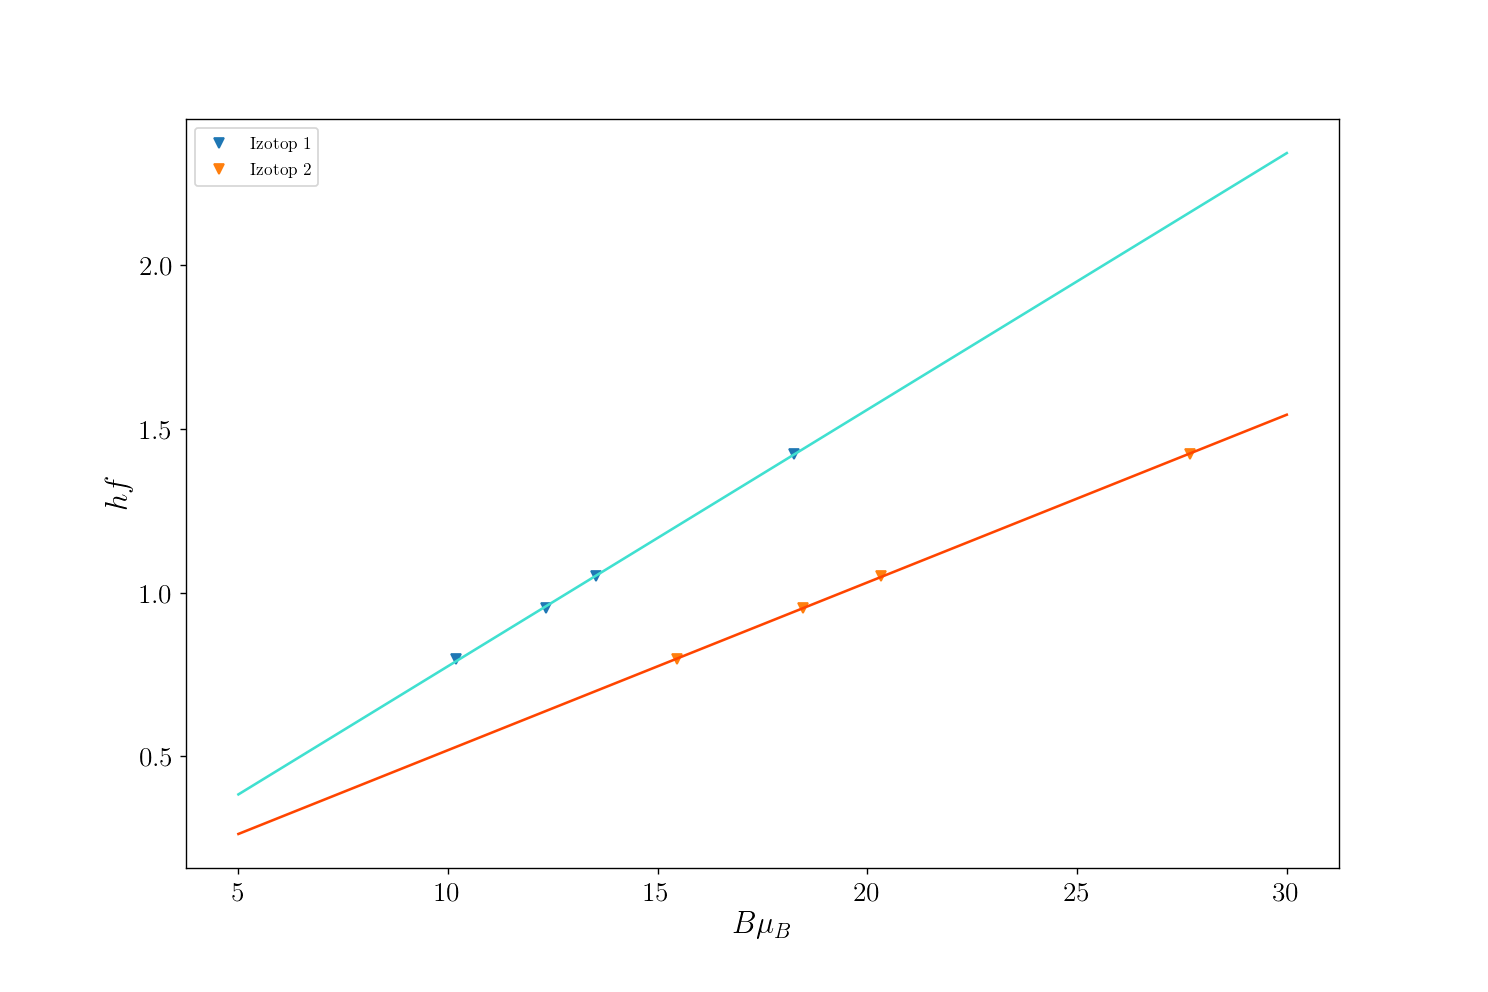
\includegraphics[width=0.99\textwidth]{j/gf2.png}
\centering
\caption{Radiofrekvenciás gerjesztő foton energiája a $B\mu_B$ függvényében}
\label{fig:3}
\end{figure}
% Végére:
\pagebreak
\section{Diszkusszió}
\par A mérést másodjára végeztük el többen is, így a jegyzőkönyveink hasonlóak, hasonló forrás alapjn dolgoztunk és az adatokat közösen értékeltük ki.

\clearpage

\bibliographystyle{plain}
\bibliography{references}

\end{document}